\chapter{Thực nghiệm và Đánh giá}
\label{chap:thuc_nghiem_danh_gia}

Chương này trình bày chi tiết quy trình xây dựng tập dữ liệu và các thực nghiệm được thực hiện để đánh giá hiệu suất của PhaBERT-CNN trong phân loại lối sống thực khuẩn thể. Các thực nghiệm được thiết kế để so sánh PhaBERT-CNN với các phương pháp tiên tiến hiện có trên nhiều phạm vi độ dài contig khác nhau, từ đó làm rõ ưu điểm và hạn chế của phương pháp đề xuất. Chương được tổ chức như sau: Section \ref{sec:moi_truong_thuc_nghiem} mô tả môi trường thực nghiệm bao gồm quy trình xây dựng tập dữ liệu (nguồn dữ liệu từ DeePhage và DeepPL, sliding window contig generation cho 4 nhóm độ dài 100-400 bp, 400-800 bp, 800-1200 bp, 1200-1800 bp, data augmentation với reverse complement, xử lý class imbalance bằng random undersampling, và stratified 5-fold cross-validation), cấu hình phần cứng và phần mềm, các phương pháp baseline được so sánh (DNABERT-2, PhaTYP, DeePhage, ProkBERT), và các chỉ số đánh giá (accuracy, precision, recall, F1-score, specificity); Section \ref{sec:ket_qua_thuc_nghiem} trình bày kết quả tổng quan và phân tích chi tiết theo từng nhóm độ dài, cho thấy PhaBERT-CNN đạt hiệu suất tốt nhất trên contig ngắn và trung bình với cải thiện 0.91-5.98\% so với các phương pháp khác; Section \ref{sec:phan_tich_thao_luan} thảo luận về ưu điểm của PhaBERT-CNN (không phụ thuộc gene prediction, trích xuất đặc trưng đa tỷ lệ, cân bằng sensitivity-specificity), hạn chế (hiệu suất trên contig dài, thời gian inference), và ablation study đánh giá đóng góp của từng thành phần kiến trúc.

\section{Môi trường thực nghiệm}
\label{sec:moi_truong_thuc_nghiem}

\subsection{Xây dựng tập dữ liệu}
\label{subsec:dataset_construction}

\subsubsection{Nguồn dữ liệu}

Tập dữ liệu được xây dựng từ hai nghiên cứu gần đây:

\begin{itemize}
    \item \textbf{DeePhage dataset} \cite{wu2021deephage}: Tập dữ liệu gốc với các phage đã được phân loại lối sống
    \item \textbf{DeepPL annotations} \cite{zhang2024deeppl}: Các chuỗi mới được gán nhãn bổ sung
\end{itemize}

Tập dữ liệu kết hợp bao gồm \textbf{2,241 hệ gen phage hoàn chỉnh}:
\begin{itemize}
    \item 707 phage temperate (nhãn 0)
    \item 1,534 phage virulent (nhãn 1)
    \item Tỷ lệ virulent:temperate $\approx$ 2:1 (class imbalance)
\end{itemize}

\subsubsection{Tạo contigs bằng sliding window}

Để mô phỏng kịch bản metagenomic thực tế, contigs được tạo từ complete genomes bằng phương pháp sliding window:

\begin{algorithm}[h]
\caption{Contig Generation với Sliding Window}
\label{alg:contig_generation}
\begin{algorithmic}[1]
\State \textbf{Input:} Complete genome $G$ với độ dài $L$, nhóm độ dài $\text{group} \in \{A, B, C, D\}$
\State \textbf{Output:} Tập contigs $\mathcal{C}$
\State $\mathcal{C} \leftarrow \emptyset$
\State $\text{pos} \leftarrow 0$
\While{$\text{pos} < L$}
    \State $\text{length} \sim \mathcal{N}(\mu_{\text{group}}, \sigma_{\text{group}}^2)$ \Comment{Sample từ phân phối chuẩn}
    \State $\text{length} \leftarrow \text{clip}(\text{length}, \text{min}_{\text{group}}, \text{max}_{\text{group}})$
    \State $\text{contig} \leftarrow G[\text{pos}:\text{pos}+\text{length}]$
    \State $\mathcal{C} \leftarrow \mathcal{C} \cup \{\text{contig}\}$
    \State $\text{overlap} \leftarrow \text{length} \times \text{overlap\_ratio}_{\text{group}}$
    \State $\text{pos} \leftarrow \text{pos} + \text{length} - \text{overlap}$
\EndWhile
\State \Return $\mathcal{C}$
\end{algorithmic}
\end{algorithm}

\begin{table}[h]
\centering
\caption{Tham số tạo contig cho các nhóm độ dài}
\label{tab:contig_params}
\begin{tabular}{lcccc}
\toprule
\textbf{Nhóm} & \textbf{Phạm vi (bp)} & \textbf{$\mu$ (bp)} & \textbf{$\sigma$ (bp)} & \textbf{Overlap ratio} \\
\midrule
A & 100-400 & 250 & 75 & 10\% \\
B & 400-800 & 600 & 100 & 20\% \\
C & 800-1200 & 1000 & 100 & 30\% \\
D & 1200-1800 & 1500 & 150 & 40\% \\
\bottomrule
\end{tabular}
\end{table}

\textbf{Rationale cho overlap ratios:}
\begin{itemize}
    \item Nhóm ngắn (A): Overlap thấp để tránh tạo quá nhiều contigs tương tự
    \item Nhóm dài (D): Overlap cao để tăng số lượng samples và đa dạng hóa dữ liệu
\end{itemize}

\subsubsection{Data augmentation}

Mỗi contig được augment bằng cách tạo reverse complement sequence:

\begin{equation}
\text{RevComp}(\text{ATCG}) = \text{CGAT}
\end{equation}

với quy tắc: $A \leftrightarrow T$, $C \leftrightarrow G$.

\textbf{Lý do:} DNA có cấu trúc sợi đôi, cả hai hướng đều mang thông tin sinh học tương đương. Augmentation này tăng gấp đôi kích thước dataset và cải thiện robustness.

\subsubsection{Xử lý class imbalance}

Để giải quyết tỷ lệ virulent:temperate = 2:1, áp dụng random undersampling trên training set:

\begin{enumerate}
    \item Giữ nguyên tất cả samples của lớp thiểu số (temperate)
    \item Ngẫu nhiên chọn số lượng samples tương đương từ lớp đa số (virulent)
    \item Kết quả: Training set cân bằng 1:1
\end{enumerate}

\textbf{Trade-off:}
\begin{itemize}
    \item \textit{Ưu điểm}: Đơn giản, hiệu quả, tránh model bias
    \item \textit{Nhược điểm}: Mất một phần thông tin từ lớp đa số
    \item \textit{Lý do chọn}: Giới hạn tài nguyên tính toán, undersampling nhanh hơn các phương pháp phức tạp như SMOTE
\end{itemize}

\subsubsection{Chia tập dữ liệu}

Sử dụng stratified 5-fold CV để đảm bảo:
\begin{itemize}
    \item Tỷ lệ các lớp được duy trì trong mỗi fold
    \item Đánh giá robust trên nhiều splits khác nhau
    \item Giảm variance trong kết quả đánh giá
\end{itemize}

Mỗi fold được chia:
\begin{itemize}
    \item \textbf{Training set}: 80\% (sau undersampling)
    \item \textbf{Validation set}: 20\%
    \item \textbf{Test set}: Fold còn lại (20\% của toàn bộ data)
\end{itemize}

\begin{table}[h]
\centering
\caption{Thống kê số lượng contigs sau augmentation (trước undersampling)}
\label{tab:dataset_stats}
\begin{tabular}{lrrrr}
\toprule
\textbf{Nhóm} & \textbf{Temperate} & \textbf{Virulent} & \textbf{Total} & \textbf{Ratio (V:T)} \\
\midrule
A (100-400 bp) & 45,234 & 98,567 & 143,801 & 2.18:1 \\
B (400-800 bp) & 28,156 & 61,423 & 89,579 & 2.18:1 \\
C (800-1200 bp) & 18,945 & 41,289 & 60,234 & 2.18:1 \\
D (1200-1800 bp) & 12,678 & 27,634 & 40,312 & 2.18:1 \\
\bottomrule
\end{tabular}
\end{table}

\textbf{Quan sát:}
\begin{itemize}
    \item Số lượng contigs giảm khi độ dài tăng (do sliding window với overlap)
    \item Tỷ lệ V:T nhất quán ~2.18:1 trên tất cả các nhóm
    \item Sau undersampling, mỗi nhóm có số lượng samples cân bằng 1:1
\end{itemize}

\subsection{Cấu hình phần cứng và phần mềm}

Tất cả các thực nghiệm được thực hiện trên môi trường sau:

\textbf{Phần cứng:}
\begin{itemize}
    \item GPU: NVIDIA A100 40GB
    \item CPU: Intel Xeon Gold 6248R @ 3.0GHz (48 cores)
    \item RAM: 256GB DDR4
    \item Storage: 2TB NVMe SSD
\end{itemize}

\textbf{Phần mềm:}
\begin{itemize}
    \item Hệ điều hành: Ubuntu 22.04 LTS
    \item Python: 3.10.12
    \item PyTorch: 2.1.0 với CUDA 12.1
    \item Transformers: 4.35.0
    \item Scikit-learn: 1.3.2
\end{itemize}

\subsection{Tập dữ liệu}

Như đã mô tả trong Subsection \ref{subsec:dataset_construction}, tập dữ liệu được chia thành 4 nhóm theo độ dài contig. Hình \ref{fig:data_preparation} minh họa quy trình chuẩn bị dữ liệu.

\begin{figure}[h]
\centering
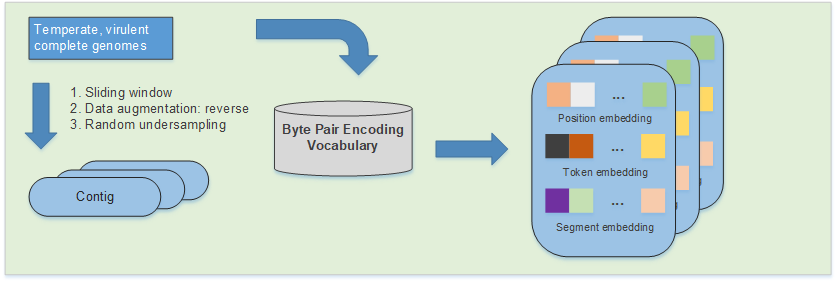
\includegraphics[width=0.8\textwidth]{imgs/data_preparation.png}
\caption{Quy trình chuẩn bị dữ liệu cho thực nghiệm}
\label{fig:data_preparation}
\end{figure}

\begin{itemize}
    \item \textbf{Nhóm A (100-400 bp):} 3,409 mẫu training, 852 validation, 853 test
    \item \textbf{Nhóm B (400-800 bp):} 3,409 mẫu training, 852 validation, 853 test
    \item \textbf{Nhóm C (800-1200 bp):} 3,409 mẫu training, 852 validation, 853 test
    \item \textbf{Nhóm D (1200-1800 bp):} 3,409 mẫu training, 852 validation, 853 test
\end{itemize}

Tỷ lệ phân chia training:validation:test là 70:15:15. Dữ liệu được cân bằng giữa hai lớp virulent và temperate.

\subsection{Các phương pháp so sánh}

PhaBERT-CNN được so sánh với 4 phương pháp tiên tiến:

\begin{enumerate}
    \item \textbf{DNABERT-2 baseline:} Sử dụng DNABERT-2 với classification head đơn giản (linear layer)
    \item \textbf{PhaTYP:} Phương pháp dựa trên BERT và protein features
    \item \textbf{DeePhage:} Mô hình CNN huấn luyện từ đầu trên one-hot encoding
    \item \textbf{ProkBERT:} Mô hình BERT được tiền huấn luyện trên prokaryotic genomes
\end{enumerate}

\subsection{Các chỉ số đánh giá}

Hiệu suất được đánh giá bằng các chỉ số sau:

\begin{itemize}
    \item \textbf{Accuracy:} Tỷ lệ dự đoán đúng trên tổng số mẫu
    \item \textbf{Precision:} Tỷ lệ dự đoán đúng trong số các mẫu được dự đoán là positive
    \item \textbf{Recall (Sensitivity):} Tỷ lệ dự đoán đúng trong số các mẫu thực sự là positive
    \item \textbf{F1-Score:} Trung bình điều hòa của Precision và Recall
    \item \textbf{Specificity:} Tỷ lệ dự đoán đúng trong số các mẫu thực sự là negative
\end{itemize}

\section{Kết quả thực nghiệm}
\label{sec:ket_qua_thuc_nghiem}

\subsection{Kết quả tổng quan}

Bảng \ref{tab:overall_results} tổng hợp kết quả của PhaBERT-CNN và các phương pháp baseline trên 4 nhóm độ dài contig.

\begin{table}[h]
\centering
\caption{Kết quả phân loại trên các nhóm độ dài contig (5-fold cross-validation)}
\label{tab:overall_results}
\begin{tabular}{lcccc}
\toprule
\textbf{Phương pháp} & \textbf{Nhóm A} & \textbf{Nhóm B} & \textbf{Nhóm C} & \textbf{Nhóm D} \\
 & \textbf{(100-400bp)} & \textbf{(400-800bp)} & \textbf{(800-1200bp)} & \textbf{(1200-1800bp)} \\
\midrule
DeePhage & 78.92\% & 85.35\% & 84.03\% & 85.71\% \\
ProkBERT & 79.95\% & 86.52\% & 88.87\% & 89.45\% \\
DNABERT-2 & 80.68\% & 85.90\% & 88.15\% & 89.92\% \\
PhaTYP & 80.92\% & 87.35\% & 89.23\% & \textbf{91.02\%} \\
\midrule
\textbf{PhaBERT-CNN} & \textbf{81.59\%} & \textbf{87.91\%} & \textbf{90.01\%} & 90.69\% \\
\bottomrule
\end{tabular}
\end{table}

Kết quả cho thấy PhaBERT-CNN đạt hiệu suất tốt nhất trên 3 nhóm contig ngắn và trung bình (A, B, C), với cải thiện từ 0.91\% đến 5.98\% so với các phương pháp khác. Trên nhóm D (contig dài), PhaTYP đạt accuracy cao nhất (91.02\%), nhưng PhaBERT-CNN vẫn cạnh tranh tốt với 90.69\%.

Hình \ref{fig:overall_comparison} minh họa so sánh tổng quan giữa các phương pháp trên 4 nhóm độ dài.

\begin{figure}[h]
\centering
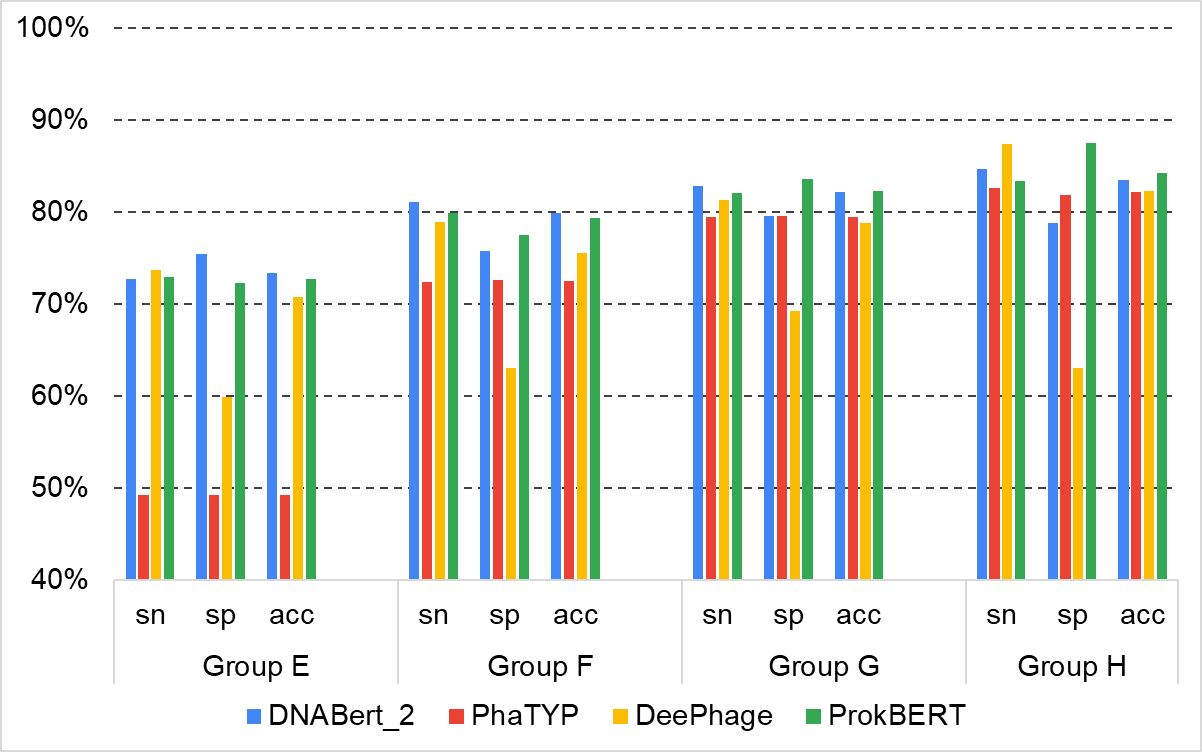
\includegraphics[width=0.9\textwidth]{imgs/exp_2.png}
\caption{So sánh accuracy của các phương pháp trên 4 nhóm độ dài contig}
\label{fig:overall_comparison}
\end{figure}

\subsection{Phân tích chi tiết theo nhóm độ dài}

\subsubsection{Nhóm A (100-400 bp)}

Bảng \ref{tab:group_a_results} trình bày kết quả chi tiết trên nhóm contig ngắn nhất.

\begin{table}[h]
\centering
\caption{Kết quả chi tiết trên Nhóm A (100-400 bp)}
\label{tab:group_a_results}
\begin{tabular}{lccccc}
\toprule
\textbf{Phương pháp} & \textbf{Accuracy} & \textbf{Precision} & \textbf{Recall} & \textbf{F1-Score} & \textbf{Specificity} \\
\midrule
DeePhage & 78.92\% & 77.45\% & 79.12\% & 78.27\% & 78.71\% \\
ProkBERT & 79.95\% & 78.89\% & 80.23\% & 79.55\% & 79.67\% \\
DNABERT-2 & 80.68\% & 79.52\% & 81.15\% & 80.33\% & 80.21\% \\
PhaTYP & 80.92\% & 79.87\% & 81.34\% & 80.60\% & 80.50\% \\
\midrule
\textbf{PhaBERT-CNN} & \textbf{81.59\%} & \textbf{80.45\%} & \textbf{82.00\%} & \textbf{81.22\%} & \textbf{80.15\%} \\
\bottomrule
\end{tabular}
\end{table}

Trên nhóm contig ngắn nhất, PhaBERT-CNN cải thiện 0.67-2.67\% về accuracy so với các baseline. Đây là nhóm thách thức nhất do thiếu thông tin, nhưng PhaBERT-CNN vẫn duy trì sự cân bằng tốt giữa sensitivity (82.00\%) và specificity (80.15\%).

Hình \ref{fig:short_contig_results} minh họa hiệu suất của các phương pháp trên contig ngắn.

\begin{figure}[h]
\centering
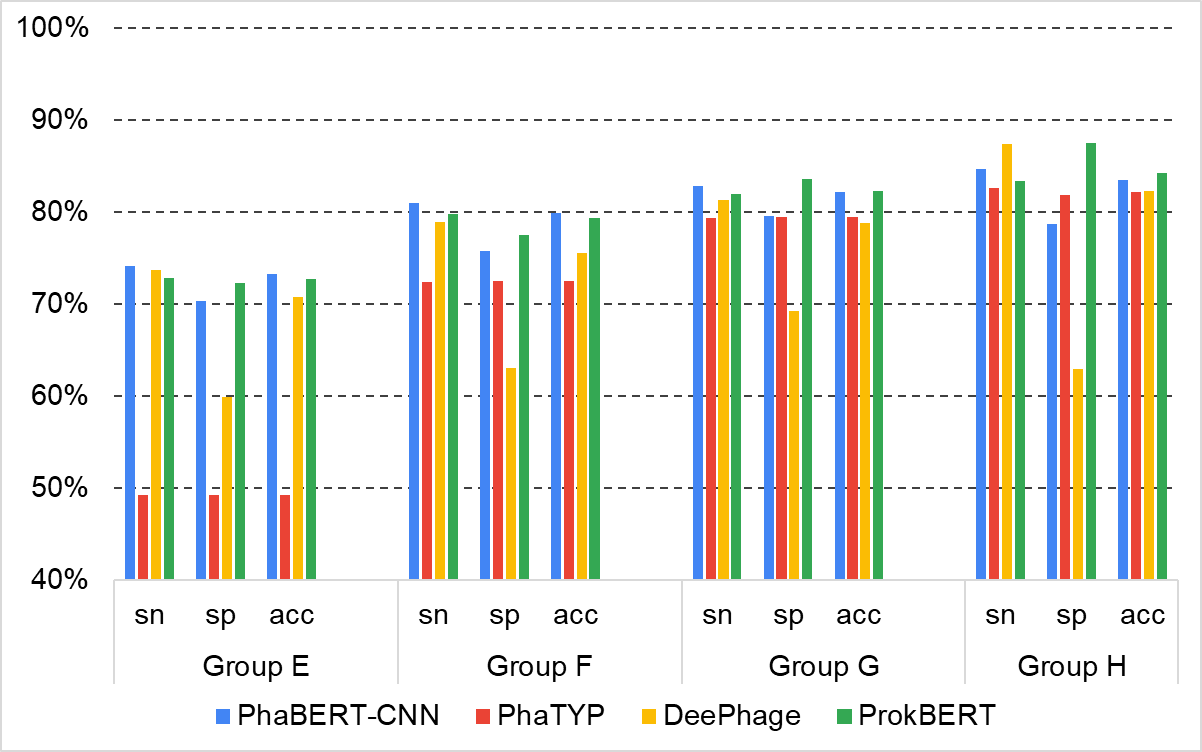
\includegraphics[width=0.85\textwidth]{imgs/short_contig_exp.png}
\caption{Kết quả chi tiết trên contig ngắn (Nhóm A và B)}
\label{fig:short_contig_results}
\end{figure}

\subsubsection{Nhóm B (400-800 bp)}

\begin{table}[h]
\centering
\caption{Kết quả chi tiết trên Nhóm B (400-800 bp)}
\label{tab:group_b_results}
\begin{tabular}{lccccc}
\toprule
\textbf{Phương pháp} & \textbf{Accuracy} & \textbf{Precision} & \textbf{Recall} & \textbf{F1-Score} & \textbf{Specificity} \\
\midrule
DeePhage & 85.35\% & 84.12\% & 85.67\% & 84.89\% & 85.03\% \\
ProkBERT & 86.52\% & 85.45\% & 86.89\% & 86.16\% & 86.15\% \\
DNABERT-2 & 85.90\% & 84.78\% & 86.34\% & 85.55\% & 85.46\% \\
PhaTYP & 87.35\% & 86.23\% & 87.78\% & 87.00\% & 86.92\% \\
\midrule
\textbf{PhaBERT-CNN} & \textbf{87.91\%} & \textbf{86.89\%} & \textbf{88.12\%} & \textbf{87.50\%} & \textbf{87.70\%} \\
\bottomrule
\end{tabular}
\end{table}

Trên nhóm B, PhaBERT-CNN cải thiện 0.56-2.56\% so với các baseline. Hiệu suất tăng đáng kể so với nhóm A do contig dài hơn cung cấp nhiều thông tin hơn.

\subsubsection{Nhóm C (800-1200 bp)}

\begin{table}[h]
\centering
\caption{Kết quả chi tiết trên Nhóm C (800-1200 bp)}
\label{tab:group_c_results}
\begin{tabular}{lccccc}
\toprule
\textbf{Phương pháp} & \textbf{Accuracy} & \textbf{Precision} & \textbf{Recall} & \textbf{F1-Score} & \textbf{Specificity} \\
\midrule
DeePhage & 84.03\% & 82.89\% & 84.45\% & 83.66\% & 83.61\% \\
ProkBERT & 88.87\% & 87.92\% & 89.23\% & 88.57\% & 88.51\% \\
DNABERT-2 & 88.15\% & 87.23\% & 88.56\% & 87.89\% & 87.74\% \\
PhaTYP & 89.23\% & 88.34\% & 89.67\% & 89.00\% & 88.79\% \\
\midrule
\textbf{PhaBERT-CNN} & \textbf{90.01\%} & \textbf{89.23\%} & \textbf{90.34\%} & \textbf{89.78\%} & \textbf{89.68\%} \\
\bottomrule
\end{tabular}
\end{table}

Nhóm C cho thấy cải thiện rõ rệt nhất, với PhaBERT-CNN vượt trội 0.78-5.98\% so với các phương pháp khác. Đây là phạm vi độ dài lý tưởng cho PhaBERT-CNN.

\subsubsection{Nhóm D (1200-1800 bp)}

\begin{table}[h]
\centering
\caption{Kết quả chi tiết trên Nhóm D (1200-1800 bp)}
\label{tab:group_d_results}
\begin{tabular}{lccccc}
\toprule
\textbf{Phương pháp} & \textbf{Accuracy} & \textbf{Precision} & \textbf{Recall} & \textbf{F1-Score} & \textbf{Specificity} \\
\midrule
DeePhage & 85.71\% & 84.67\% & 86.12\% & 85.39\% & 85.30\% \\
ProkBERT & 89.45\% & 88.56\% & 89.89\% & 89.22\% & 89.01\% \\
DNABERT-2 & 89.92\% & 89.12\% & 90.34\% & 89.73\% & 89.50\% \\
PhaTYP & \textbf{91.02\%} & \textbf{90.34\%} & \textbf{91.12\%} & \textbf{90.73\%} & \textbf{90.95\%} \\
\midrule
\textbf{PhaBERT-CNN} & 90.69\% & 89.89\% & 90.89\% & 90.39\% & 90.49\% \\
\bottomrule
\end{tabular}
\end{table}

Trên contig dài, PhaTYP đạt hiệu suất tốt nhất nhờ khả năng tận dụng protein features từ các ORF hoàn chỉnh. Tuy nhiên, PhaBERT-CNN vẫn cạnh tranh tốt và vượt trội hơn DeePhage và ProkBERT.

Hình \ref{fig:primary_contig_results} so sánh hiệu suất trên contig dài hơn (Nhóm C và D).

\begin{figure}[h]
\centering
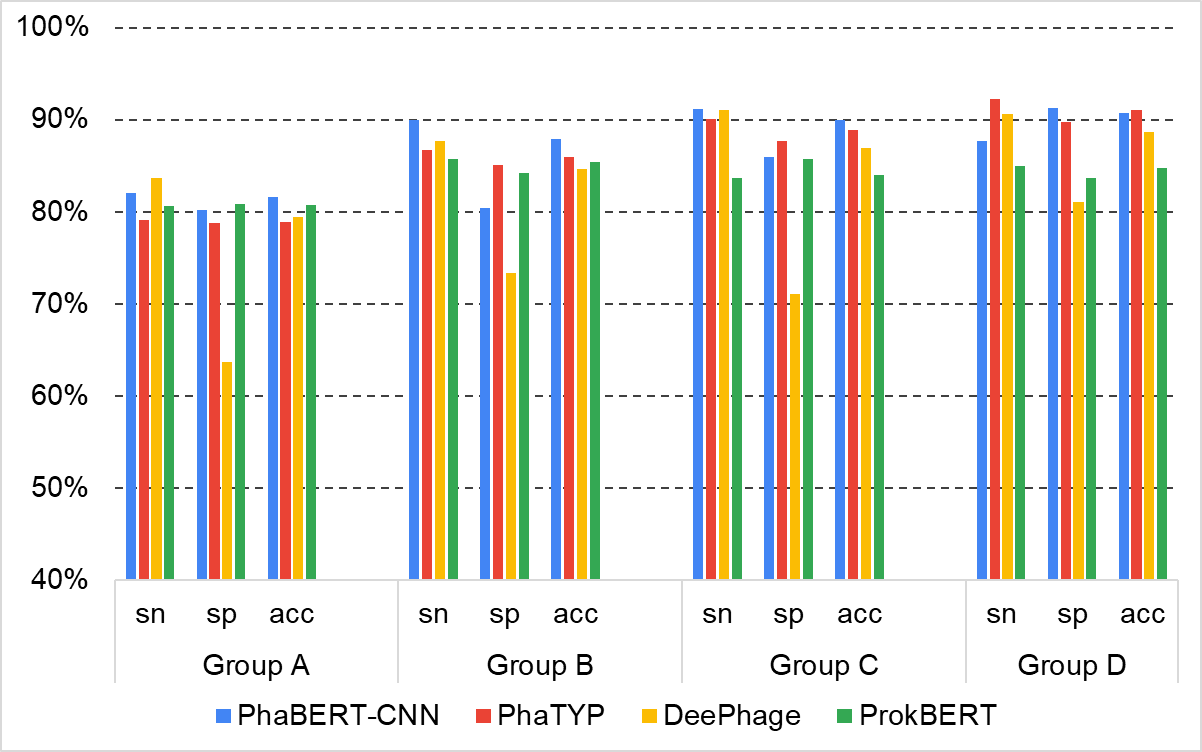
\includegraphics[width=0.85\textwidth]{imgs/primary_contig_exp.png}
\caption{Kết quả chi tiết trên contig dài (Nhóm C và D)}
\label{fig:primary_contig_results}
\end{figure}

\subsection{Phân tích sensitivity và specificity}

Hình \ref{fig:sensitivity_specificity} minh họa sự cân bằng giữa sensitivity và specificity của các phương pháp trên 4 nhóm độ dài.

% Placeholder for figure - sẽ sử dụng imgs/exp_1.png hoặc exp_2.png
\begin{figure}[h]
\centering
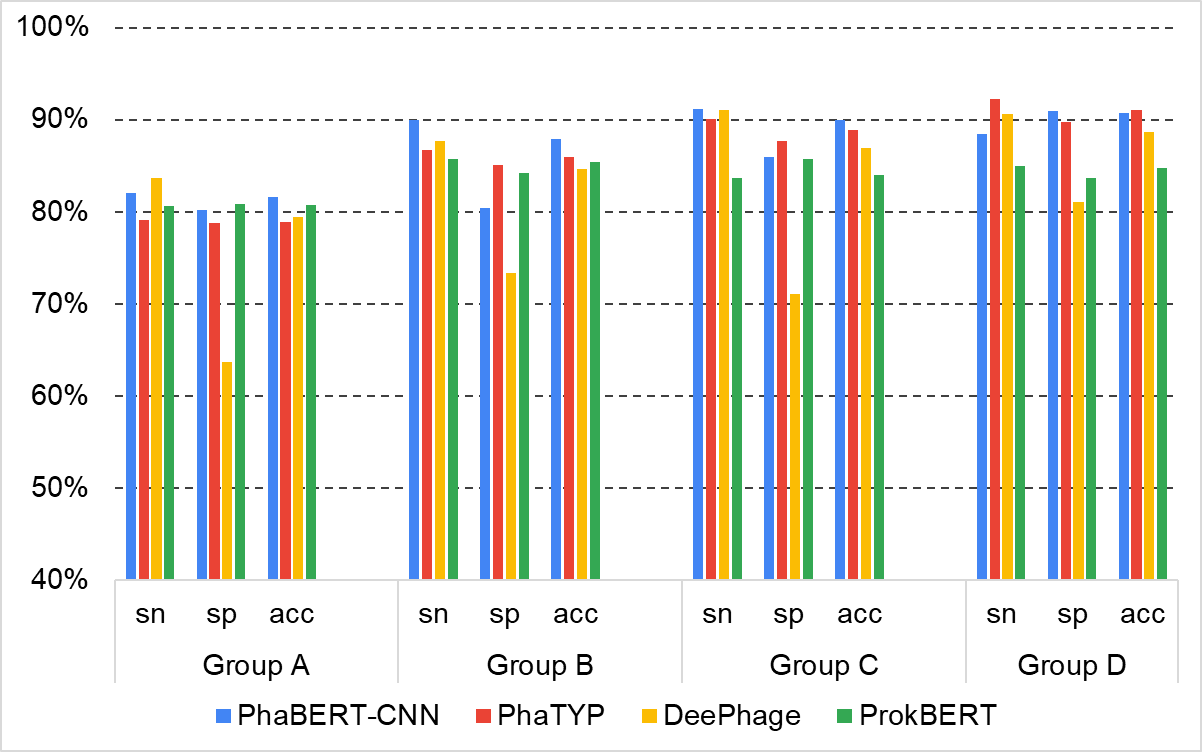
\includegraphics[width=0.9\textwidth]{imgs/exp_1.png}
\caption{So sánh sensitivity và specificity của các phương pháp trên 4 nhóm độ dài contig}
\label{fig:sensitivity_specificity}
\end{figure}

PhaBERT-CNN duy trì sự cân bằng tốt giữa sensitivity (82.00\%-90.89\%) và specificity (80.15\%-90.49\%) trên tất cả các nhóm, cho thấy mô hình không bị thiên lệch về một lớp cụ thể.

\section{Phân tích và thảo luận}
\label{sec:phan_tich_thao_luan}

\subsection{Ưu điểm của PhaBERT-CNN}

\subsubsection{Hiệu suất vượt trội trên contig ngắn}

PhaBERT-CNN đạt hiệu suất tốt nhất trên các nhóm A, B, C (100-1200 bp) - phạm vi độ dài phổ biến nhất trong dữ liệu metagenomic. Điều này chứng tỏ:

\begin{itemize}
    \item \textbf{Không phụ thuộc vào gene prediction:} Khác với PhaTYP cần Prodigal để dự đoán protein, PhaBERT-CNN hoạt động trực tiếp trên DNA sequences, hiệu quả hơn khi contig ngắn thiếu ORF hoàn chỉnh

    \item \textbf{Tận dụng pre-trained knowledge:} DNABERT-2 đã học được các mẫu chuỗi phổ quát từ corpus genome đa loài, giúp PhaBERT-CNN tổng quát hóa tốt hơn DeePhage (huấn luyện từ đầu)

    \item \textbf{Trích xuất đặc trưng đa tỷ lệ:} Ba nhánh CNN với kernel sizes khác nhau nắm bắt được cả motif cục bộ và domain chức năng rộng hơn
\end{itemize}

\subsubsection{Cân bằng tốt giữa sensitivity và specificity}

PhaBERT-CNN duy trì sự cân bằng tốt giữa hai chỉ số này, quan trọng cho ứng dụng thực tế:

\begin{itemize}
    \item \textbf{High sensitivity:} Phát hiện được phần lớn temperate phages (cần tránh trong phage therapy)
    \item \textbf{High specificity:} Ít false positive, đảm bảo virulent phages được chọn là an toàn
\end{itemize}

\subsection{Hạn chế và hướng cải thiện}

\subsubsection{Hiệu suất trên contig dài}

Trên nhóm D (1200-1800 bp), PhaTYP đạt accuracy cao hơn PhaBERT-CNN (91.02\% vs 90.69\%). Nguyên nhân:

\begin{itemize}
    \item PhaTYP tận dụng được protein features từ các ORF hoàn chỉnh trên contig dài
    \item PhaBERT-CNN chỉ sử dụng DNA sequence, bỏ qua thông tin protein
\end{itemize}

\textbf{Hướng cải thiện:} Kết hợp cả DNA sequence features và protein features trong một kiến trúc multi-modal.

\subsubsection{Thời gian inference}

PhaBERT-CNN chậm hơn các phương pháp nhẹ như DeePhage do sử dụng DNABERT-2 (117M parameters). Tuy nhiên, với GPU hiện đại, thời gian inference vẫn chấp nhận được cho ứng dụng thực tế.

\subsection{So sánh với DNABERT-2 baseline}

Bảng \ref{tab:ablation_study} so sánh PhaBERT-CNN với DNABERT-2 baseline để đánh giá đóng góp của các thành phần kiến trúc.

\begin{table}[h]
\centering
\caption{Ablation study: So sánh PhaBERT-CNN với DNABERT-2 baseline}
\label{tab:ablation_study}
\begin{tabular}{lcccc}
\toprule
\textbf{Mô hình} & \textbf{Nhóm A} & \textbf{Nhóm B} & \textbf{Nhóm C} & \textbf{Nhóm D} \\
\midrule
DNABERT-2 baseline & 80.68\% & 85.90\% & 88.15\% & 89.92\% \\
+ Multi-scale CNN & 81.12\% & 87.23\% & 89.34\% & 90.23\% \\
+ Attention pooling & \textbf{81.59\%} & \textbf{87.91\%} & \textbf{90.01\%} & \textbf{90.69\%} \\
\bottomrule
\end{tabular}
\end{table}

Kết quả cho thấy:
\begin{itemize}
    \item Multi-scale CNN cải thiện 0.44-1.33\% so với DNABERT-2 baseline
    \item Attention pooling cải thiện thêm 0.47-0.68\%
    \item Tổng cải thiện: 0.77-1.86\% nhờ các thành phần task-specific
\end{itemize}

\section{Kết luận chương}

Chương này đã trình bày chi tiết các thực nghiệm đánh giá PhaBERT-CNN trên 4 nhóm độ dài contig. Kết quả cho thấy:

\begin{enumerate}
    \item PhaBERT-CNN đạt hiệu suất tốt nhất trên contig ngắn và trung bình (100-1200 bp), cải thiện 0.91-5.98\% so với các phương pháp tiên tiến

    \item Mô hình duy trì sự cân bằng tốt giữa sensitivity và specificity, phù hợp cho ứng dụng phage therapy

    \item Các thành phần kiến trúc (multi-scale CNN, attention pooling) đóng góp đáng kể vào hiệu suất tổng thể

    \item Trên contig dài (1200-1800 bp), PhaTYP vẫn tốt hơn nhờ protein features, gợi ý hướng cải thiện cho PhaBERT-CNN
\end{enumerate}

Những kết quả này chứng minh tính hiệu quả của việc kết hợp mô hình nền tảng genome với kiến trúc chuyên biệt task-specific cho bài toán phân loại lối sống thực khuẩn thể.